\documentclass[a4paper,12pt]{article}

% Need \centerdot
\usepackage{amssymb}

% Set margins
\usepackage{geometry}
\geometry{
  top=1.0cm,            % <-- you want to adjust this
  inner=1.5cm,
  outer=1.5cm,
  bottom=1.0cm,
  headheight=3ex,       % <-- and this
  headsep=2ex,          % <-- and this
}

% No page numbers
\pagestyle{empty}

% Set paragraph indent to 2.2mm, even first
\usepackage{indentfirst}
\setlength{\parindent}{2.2mm}

% Image support
\usepackage{graphicx}

% Need \XeLaTex logo
\usepackage{xltxtra}

% Set font to Garamond
\usepackage{fontspec}
\setmainfont[Numbers=OldStyle,
	     Scale=1.05,
	     ItalicFont={Adobe Garamond Pro Italic},
             BoldFont={Adobe Garamond Pro Semibold}
            ]{Adobe Garamond Pro}

% Set section to MidnightBlue with horizontal rule
\usepackage[dvipsnames,usenames]{color}
\usepackage[explicit]{titlesec}
\titleformat{\section}[display]{\Large\color{MidnightBlue}}{\thetitle}{1em}{#1}[{\titlerule}]

% Text layout commands
\newcommand{\topSection}[2]
{
	\begin{minipage}[b]{0.68\textwidth} #1 \end{minipage}
	\begin{minipage}[t]{0.28\textwidth} #2 \end{minipage}
	\vspace{0.4\baselineskip}
}

\newcommand{\standardEntry}[2]
{
	\vspace{0.4\baselineskip}
	\begin{minipage}[t]{0.25\textwidth} {\small \textsc{#1}} \end{minipage}
	\begin{minipage}[t]{0.725\textwidth} #2 \end{minipage}
	\par
}

\newcommand{\stretchedEntry}[2]
{
	\vspace{0.4\baselineskip}
	#1 \hfill #2
	\vspace{\baselineskip}
	\par
}

\newcommand{\indentedEntry}[2]
{
	\standardEntry{\hspace{0.125\textwidth} #1}{#2}
}


\begin{document}

\topSection
{
	{\Huge Jorge Azevedo}

	\vspace{1.5mm}

	\resizebox{4.9cm}{!}{\textit{Electronics Engineer}}

	\vspace*{10mm}

	\textbf{Availability}: July 2013 onwards

	\textbf{Looking for}: Real-Time Linux

	\hspace{66pt}Embedded Systems Development

	\textbf{E-mail}: jorge.amado.azevedo@gmail.com

	\textbf{Tel}: \small{(+351) 936270876}
} {
	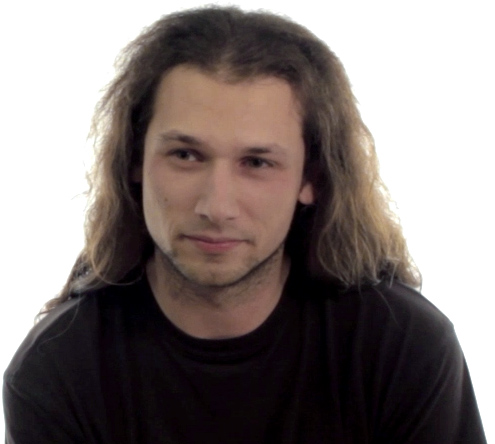
\includegraphics[width=\textwidth]{img/foto}
}

\emph{In a nuthsell} $\cdot$  Recent university graduate passionate about
technology looking for a challenge and an opportunity to learn
a new language.  Specialties include Real-Time Linux and software development.

\section*{Personal Information}

\standardEntry{Full name}{Jorge Manuel Coelho Amado de Azevedo}
\standardEntry{Address}{Rua Bartolomeu Dias, 210, 4450-587 Matosinhos,
Portugal}
\standardEntry{Date of Birth}{15th October 1987} 
\standardEntry{Age}{25}
\standardEntry{Gender}{Male} 
\standardEntry{Nationality}{Portuguese} 
\standardEntry{Telephone}{(+351) 936270876}
\standardEntry{E-mail}{jorge.amado.azevedo@gmail.com} 
\standardEntry{LinkedIn}{pt.linkedin.com/in/jaazevedo}
\standardEntry{Xing}{Jorge Azevedo}

\section*{Experience}

\stretchedEntry{UNISOL}{Universidade de Aveiro, Portugal}
\indentedEntry{Mar 2012 - Present}{\textbf{Researcher}}
\indentedEntry{Description}
{
Research grant to work for UNISOL, an European consortium assembled
to build a domestic solar heating system from the ground up. My
responsabilities and projects included:

 $\cdot$  Prototyping an embedded control system based on a PIC32 microcontroller and
several sensors and actuators.

 $\cdot$  Development of a system simulation model using MATLAB and Simulink.

 $\cdot$  Deployment and admnistration of a Linux server running an OpenStack cloud
computing environment, a MATLAB computation clusters, and other key services.
}

\stretchedEntry{Xenomai Lab}{Universidade de Aveiro, Portugal}
\indentedEntry{Jan 2011 - Present}{\textbf{Software Engineer}}
\indentedEntry{Description}
{
Principal developer and maintainer of the Xenomai Lab real-time control
platform. This included up-close work on areas such as

 $\cdot$ Distributed version control using git.

 $\cdot$ Graphical User Interface development using Qt/C++.

 $\cdot$ The Xenomai real-time framework and its real-time semantics in C.

 $\cdot$ Licencing, packaging and distribution of a free software project.

}
\indentedEntry{Jan 2012 - Present}{\textbf{Master Thesis Colaborator}}
\indentedEntry{Description}{
Technical coordinator for several student master thesis

 $\cdot$ Sep 2012 - Present \emph{TODO}.

 $\cdot$ Jan 2012 - Dez 2012 \emph{Controlador Adaptativo baseado em Xenomai}.
}

\section*{Publications}

\standardEntry{September 2012}{Xenomai Lab - A Platform for Digital Real-Time Control}
\standardEntry{In}{INForum 2012 Procedings}

\section*{Education}

\standardEntry{2005–2012}{\textbf{M.Sc. Electronics and Telecommunications
Engineering}}
\standardEntry{Institution}
{
\textbf{Universidade de Aveiro}

Campus Universitário de Santiago, 3810-193 Aveiro, Portugal
}
\standardEntry{Thesis}{Xenomai Lab - A Platform For Digital Real-Time Control}
\standardEntry{Description}
{
5 year degree (Bachelor and Master's included).

Thesis graded 19/20 after public defense. 
}

\vspace{\baselineskip}

\standardEntry{2008–2009}{\textbf{Erasmus Exchange Program}}
\standardEntry{Institution}
{
\textbf{TU\textbackslash e Technische Universiteit Eindhoven}

Den Dolech 2, 5612 AZ Eindhoven, Netherlands
}
\standardEntry{Description}
{
One year spent abroad under the Erasmus Exchange Program.
}

\section*{Languages}

\standardEntry{Portuguese}{Native speaker}
\standardEntry{English}
{
Advanced speaker. Five years of education in the British Council achieving
level A in First Certificate of English (2001) and level B in Certificate of
Advanced English (2004)
}
\standardEntry{Spanish}{Basic understanding in both written and spoken form.}


\section*{Technical Skills}

\standardEntry{Software}
{

Advanced knowledge of C.

Working knowledge of C++ and the Qt GUI framework, Linux kernel internals.

In depth understanding of Real-Time Operating Systems based on Linux such as Xenomai, RTAI and RTLinux.

Experience in Test Driven Development, Continuous Integration and cloud computing.

}
\standardEntry{Hardware}
{
A working knowledge of PIC microcontrollers, basic analog filter design and PCB prototyping using EAGLE.
}

\section*{Soft Skills}

\standardEntry{Social Skills}
{
Experience in multicultural environments

Open-Minded

Highly responsible and professional
}
\standardEntry{Organizational Skills}
{
Independent research

Strong drive for initiative

Planning and scheduling of team/individual project.
}

\section*{Additional Skills}

\standardEntry{Driving License}{Category B-1}

\end{document}
